\chapter{Experiments and Results}

\section{Experimental Setup}

All reported metrics are computed on the temporal test partition of the pneumonia cohort (1{,}075 studies), with a positive fraction of 0.453. Patient-level bootstrap summaries are based on 887 unique \texttt{subject\_id} values. Discrimination metrics are evaluated on the full test set, while operational metrics use a fixed probability threshold of 0.5. Image and multimodal models correspond to the \texttt{stronger\_lr\_v3} configuration, and clinical baselines correspond to the \texttt{strong\_v2} artifacts. Paired comparisons use identical alignment keys (\texttt{subject\_id}, \texttt{study\_id}) across merged prediction tables.

This evaluation setup is intentionally shared across all model families so that differences in performance can be attributed to model design and input modality rather than to changes in cohort definition, label policy, or split construction. In other words, the results reported in this chapter are meant to answer a controlled comparative question: how much predictive value is obtained from triage data alone, from chest radiographs alone, and from early fusion of both modalities under the same temporally constrained benchmark?

\section{Main Results}

Table~\ref{tab:main_results} reports AUROC, AUPRC, accuracy, precision, recall, and F1 on the test split. The image-only DenseNet121 model achieves the highest AUROC (0.746), AUPRC (0.724), accuracy (0.678), recall (0.659), and F1 (0.650). The multimodal model ranks second on AUROC (0.736) and AUPRC (0.714), and third on accuracy (0.670), recall (0.606), and F1 (0.624).

Both deep learning models substantially outperform the clinical baselines on AUROC and AUPRC. Clinical XGBoost slightly exceeds logistic regression across all reported metrics. At a threshold of 0.5, multimodal precision (0.644) is marginally higher than image precision (0.641), while image recall exceeds multimodal recall (0.659 versus 0.606).

\begin{table}[htbp]
\centering
\caption{Test-set performance at probability threshold 0.5. Values are point estimates on 1{,}075 studies.}
\label{tab:main_results}
\begin{tabular}{lcccccc}
\hline
Model & AUROC & AUPRC & Accuracy & Precision & Recall & F1 \\
\hline
Clinical logistic & 0.606 & 0.548 & 0.577 & 0.535 & 0.507 & 0.521 \\
Clinical XGBoost & 0.611 & 0.567 & 0.579 & 0.535 & 0.528 & 0.532 \\
Image DenseNet121 & 0.746 & 0.724 & 0.678 & 0.641 & 0.659 & 0.650 \\
Multimodal & 0.736 & 0.714 & 0.670 & 0.644 & 0.606 & 0.624 \\
\hline
\end{tabular}
\end{table}

\begin{figure}[htbp]
    \centering
    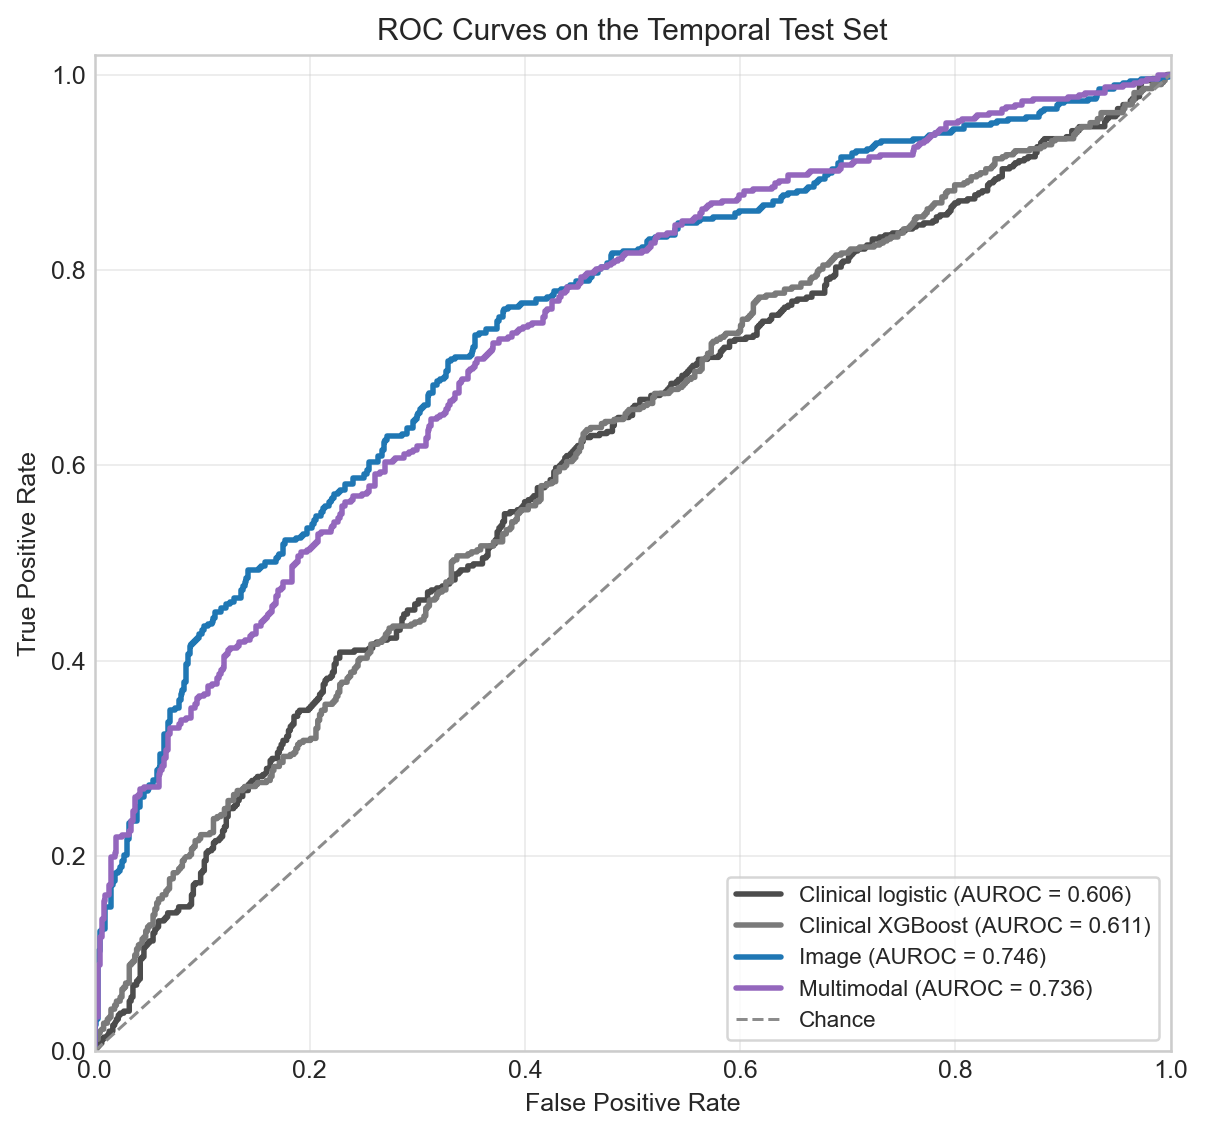
\includegraphics[width=0.8\textwidth]{images/roc_curve_all_models.png}
    \caption{Receiver operating characteristic (ROC) curves for the four evaluated models on the temporal test set. The image-only model achieves the highest discrimination performance (AUROC = 0.746), followed closely by the multimodal model (AUROC = 0.736), while both deep learning approaches substantially outperform the clinical baselines.}
    \label{fig:roc_all_models}
\end{figure}

The ROC curves for all evaluated models are shown in Figure~\ref{fig:roc_all_models}. The image-only model achieves the highest discrimination performance (AUROC = 0.746), with the multimodal model performing slightly worse (AUROC = 0.736).

Both deep learning approaches substantially outperform the clinical baselines (logistic regression: 0.606, XGBoost: 0.611). Importantly, the addition of clinical features via early fusion does not improve performance over the image-only model. This is the central empirical result of the thesis: under the current cohort design, label definition, and timing constraints, a strong radiograph model captures most of the useful signal available for the task.

The main result is therefore not simply that multimodal learning ``works,'' but that its benefit is limited in this setting. The multimodal model performs competitively in absolute terms and clearly exceeds the clinical-only baselines, yet it does not surpass the image-only baseline. This distinction is important because it shifts the interpretation from ``multimodal is better'' to ``multimodal should be justified empirically rather than assumed to be advantageous.''

\section{Uncertainty and Paired Comparisons}

Patient-level bootstrap with 2{,}000 replicates (seed 42) was applied to test predictions. For multimodal versus image, the mean paired differences were approximately $-0.0091$ AUROC (standard deviation $\approx 0.0070$) and $-0.0099$ AUPRC (standard deviation $\approx 0.0072$). The 95\% bootstrap intervals were $[-0.0227, 0.0047]$ for AUROC and $[-0.0240, 0.0040]$ for AUPRC, both including zero. The fraction of bootstrap replicates with strictly positive differences (multimodal $>$ image) was 0.10 for AUROC and 0.083 for AUPRC.

For multimodal versus clinical XGBoost, mean paired differences were approximately 0.126 AUROC and 0.147 AUPRC, with bootstrap intervals of $[0.090, 0.164]$ and $[0.104, 0.189]$, respectively. For image versus clinical XGBoost, mean paired differences were approximately 0.135 AUROC and 0.157 AUPRC, with intervals of $[0.096, 0.174]$ and $[0.112, 0.202]$. In both comparisons, all bootstrap replicates yielded strictly positive differences. No paired bootstrap comparison between clinical logistic regression and the image or multimodal models is available in the stored artifacts.

These paired comparisons strengthen the interpretation of the point estimates reported above. The image-only and multimodal models are close enough in absolute performance that one could be tempted to treat them as approximately equivalent. However, the paired bootstrap shows more specifically that there is no reliable evidence, under repeated patient-level resampling, that multimodal fusion provides a systematic improvement over the image-only model. By contrast, both image-based models clearly and consistently outperform the tabular XGBoost baseline under the same patient-level resampling procedure.

From a thesis perspective, this analysis is important because it moves beyond simple ranking by point estimate. Instead of relying only on ``0.746 is greater than 0.736,'' the paired bootstrap asks whether the observed gap is stable under resampling of the patient population. In this case, the answer is no for multimodal versus image, but clearly yes for either image-based model versus the clinical baseline. The reported fraction of bootstrap replicates in which one model exceeds another should be interpreted as a descriptive bootstrap proportion rather than as a formal frequentist \(p\)-value.

\section{Additional Analyses}

Calibration was evaluated using Brier score and expected calibration error (ECE) with ten equal-width bins and 2{,}000 bootstrap resamples. Brier scores were 0.242 (clinical logistic), 0.241 (clinical XGBoost), 0.206 (image), and 0.207 (multimodal). ECE values were 0.037, 0.046, 0.067, and 0.040, respectively. Maximum calibration error (MCE) was 0.489, 0.289, 0.165, and 0.131. Bootstrap intervals for these metrics are recorded in the calibration artifacts.

\begin{figure}[htbp]
    \centering
    
\includegraphics[width=0.8\textwidth]{images/reliability_diagram_all_models.png}
    \caption{Reliability diagram for all models on the temporal test set. The multimodal model exhibits lower expected calibration error than the image-only model, while both clinical baselines show lower discrimination and different calibration behavior.}
    \label{fig:calibration_all_models}
\end{figure}

The reliability curves for all models are shown in Figure~\ref{fig:calibration_all_models}. The multimodal model exhibits lower expected calibration error than the image-only model, as reflected by ECE values of 0.040 and 0.067, respectively.

At the same time, calibration ranking depends on the metric used. The image-only model has a slightly lower Brier score than the multimodal model (0.206 versus 0.207, rounded), while the multimodal model has lower ECE and MCE. This indicates that the two models differ not only in discrimination but also in the way their predicted probabilities are distributed across the probability range. In particular, the image-only model appears to rank cases better overall, whereas the multimodal model yields somewhat better-aligned probabilities under the fixed-bin calibration analysis.

These findings highlight that discrimination and calibration capture different aspects of model behavior. A model may separate positive and negative cases well while still producing probability estimates that are too extreme or insufficiently aligned with empirical event rates. For a thesis focused on rigorous evaluation rather than on maximizing a single headline metric, this distinction is important: better discrimination does not automatically imply better probabilistic reliability.

Decision curve analysis was computed over 99 probability thresholds between 0.01 and 0.99.

\begin{figure}[htbp]
    \centering
    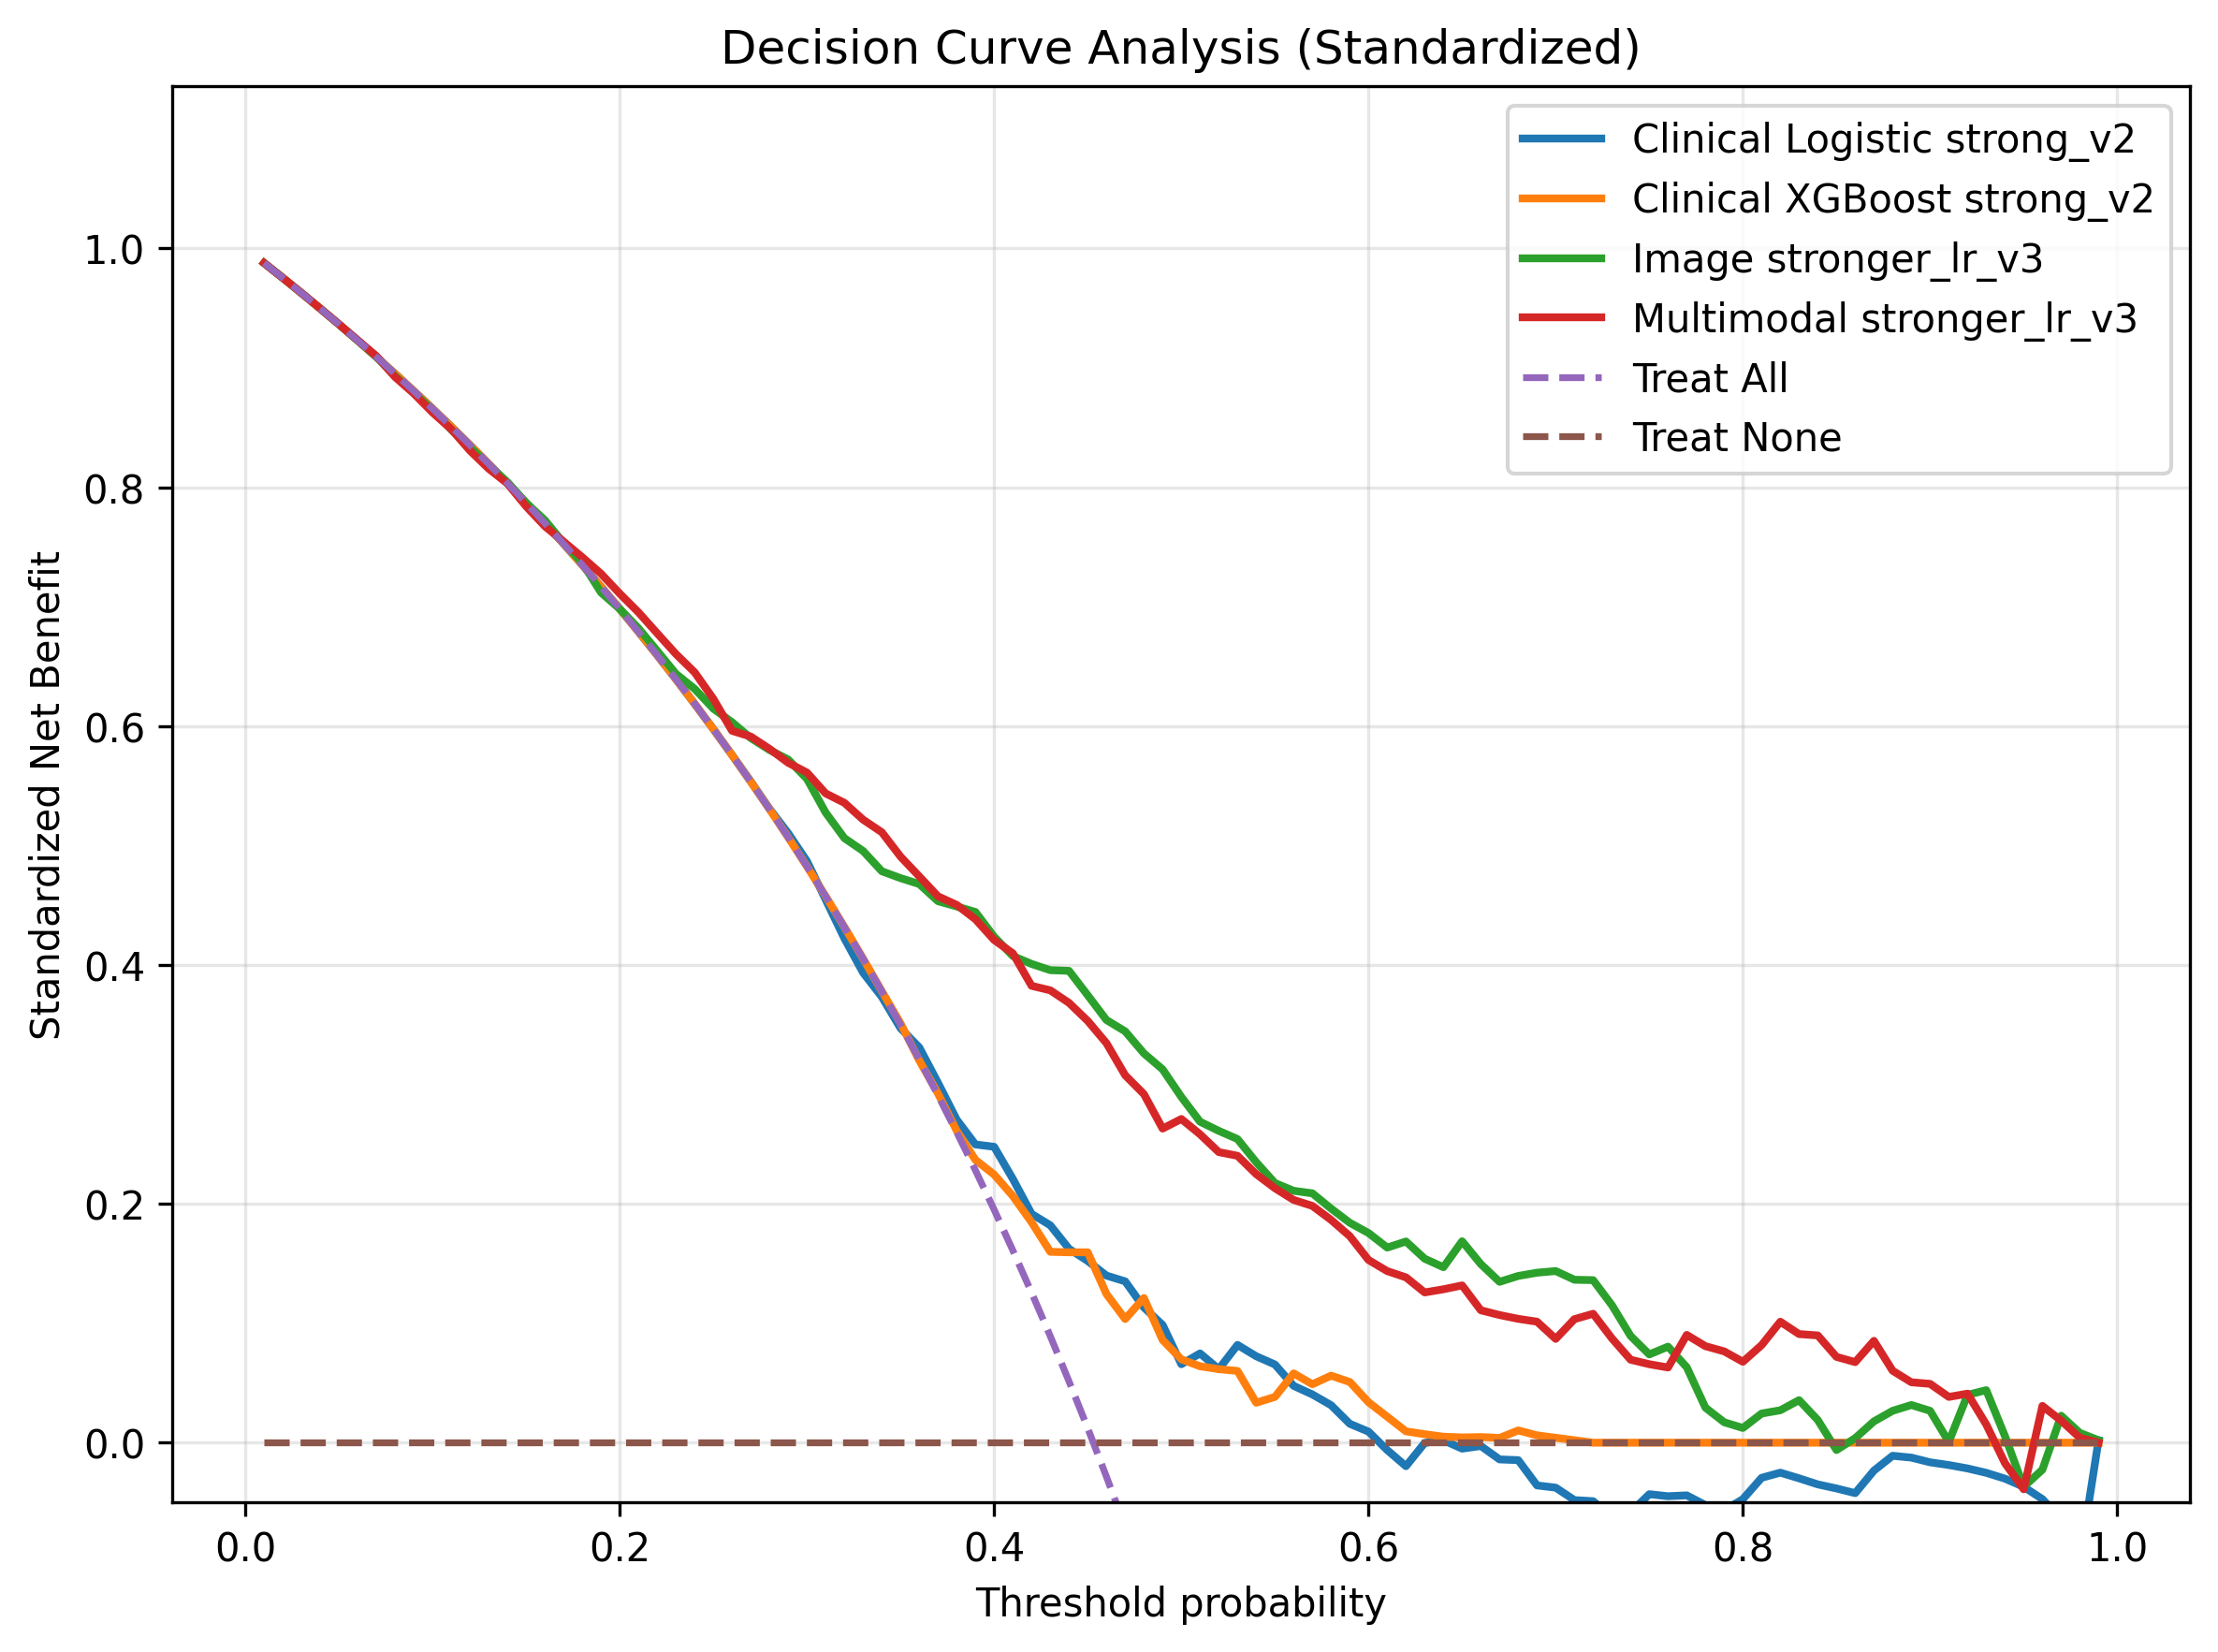
\includegraphics[width=0.8\textwidth]{images/decision_curve_standardized.png}
    \caption{Decision curve analysis for all models on the temporal test set. Both image-based models provide substantially greater net benefit than the clinical baselines, while the relative ordering of image-only and multimodal models depends on the operating threshold.}
    \label{fig:dca_all_models}
\end{figure}

Figure~\ref{fig:dca_all_models} shows that both image-based models provide substantially greater net benefit than the clinical baselines across the evaluated thresholds. The relative ordering of the image-only and multimodal models is threshold-dependent: the image model is higher at some thresholds, whereas the multimodal model is slightly higher at others. This pattern is consistent with the broader finding that multimodal fusion remains competitive but does not establish a clear overall advantage over the image-only baseline.

At a threshold of 0.5, net benefit values were approximately 0.030 (clinical logistic), 0.032 (clinical XGBoost), 0.131 (image), and 0.123 (multimodal). Full curves and tabulated results are available in the evaluation outputs.

Unlike AUROC or AUPRC, decision curve analysis translates predictive performance into a threshold-dependent utility perspective. In the present context, the DCA results reinforce two points. First, both deep learning models are substantially more useful than the triage-only baselines when decisions are made using a thresholded risk score. Second, the practical difference between image-only and multimodal systems depends on the selected threshold, rather than supporting a universal winner across all operating conditions.

\section{Qualitative Analysis}

To complement quantitative evaluation, qualitative analysis was performed using gradient-based class activation mapping (Grad-CAM) applied to representative predictions from the image model. This method highlights spatial regions that contribute most strongly to model predictions and serves as a qualitative diagnostic rather than a standalone validation method.

\begin{figure}[htbp]
    \centering

    \begin{minipage}{0.48\textwidth}
        \centering
        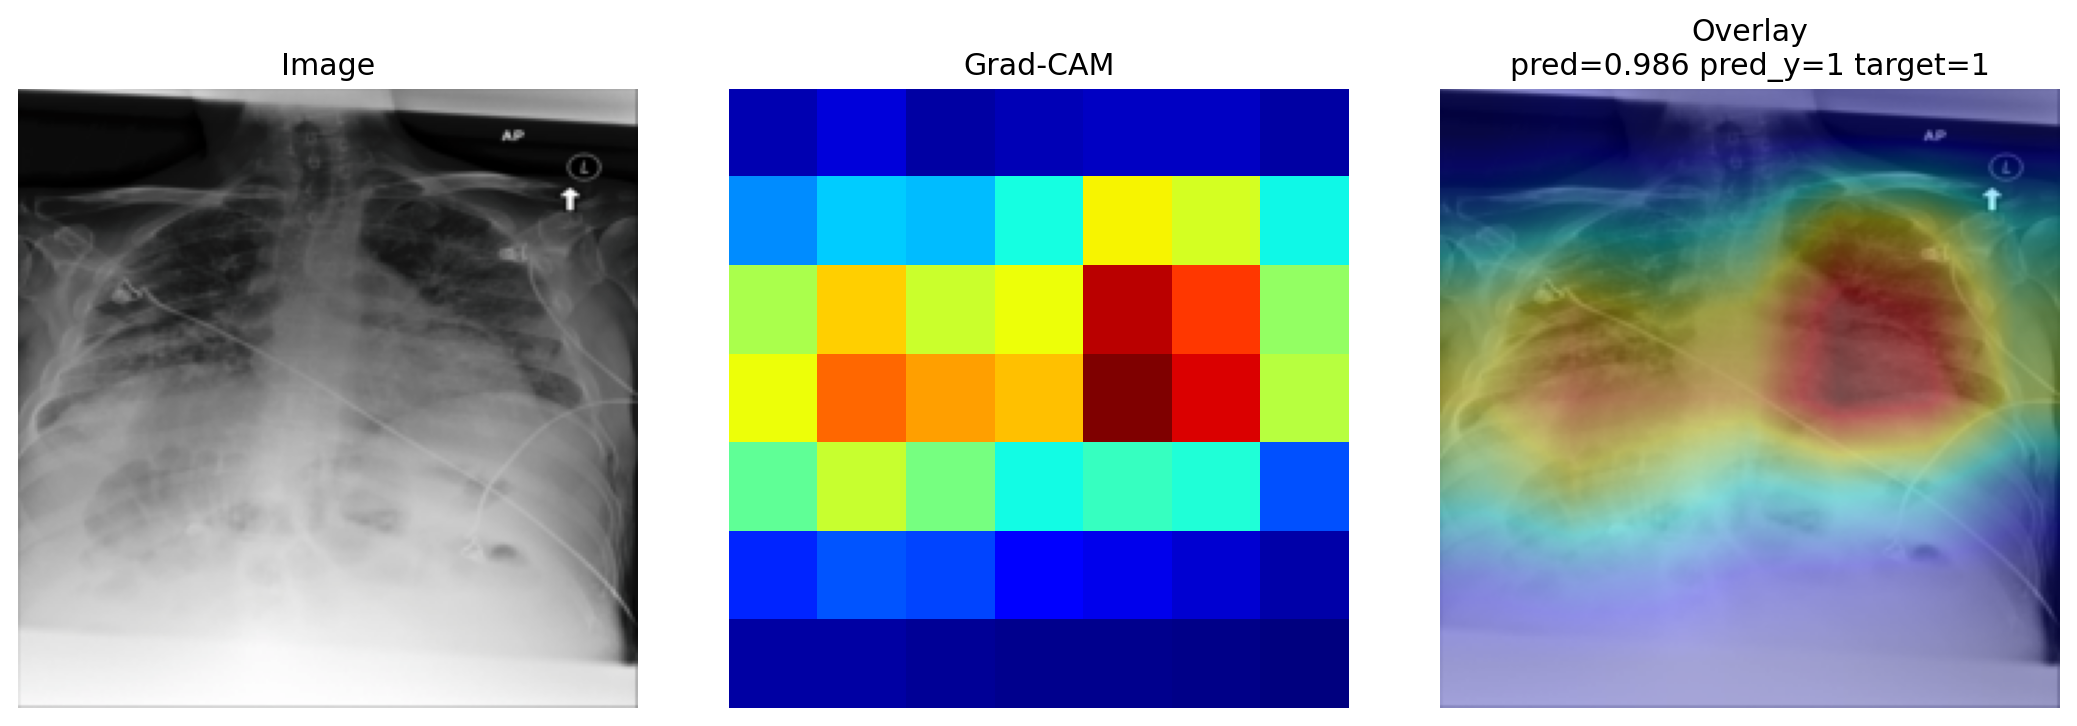
\includegraphics[width=\textwidth]{images/gradcam_tp1.png}
        \vspace{2pt}
        \small (a) True positive. Activation focuses on lower lung regions consistent with pneumonia.
    \end{minipage}
    \hfill
    \begin{minipage}{0.48\textwidth}
        \centering
        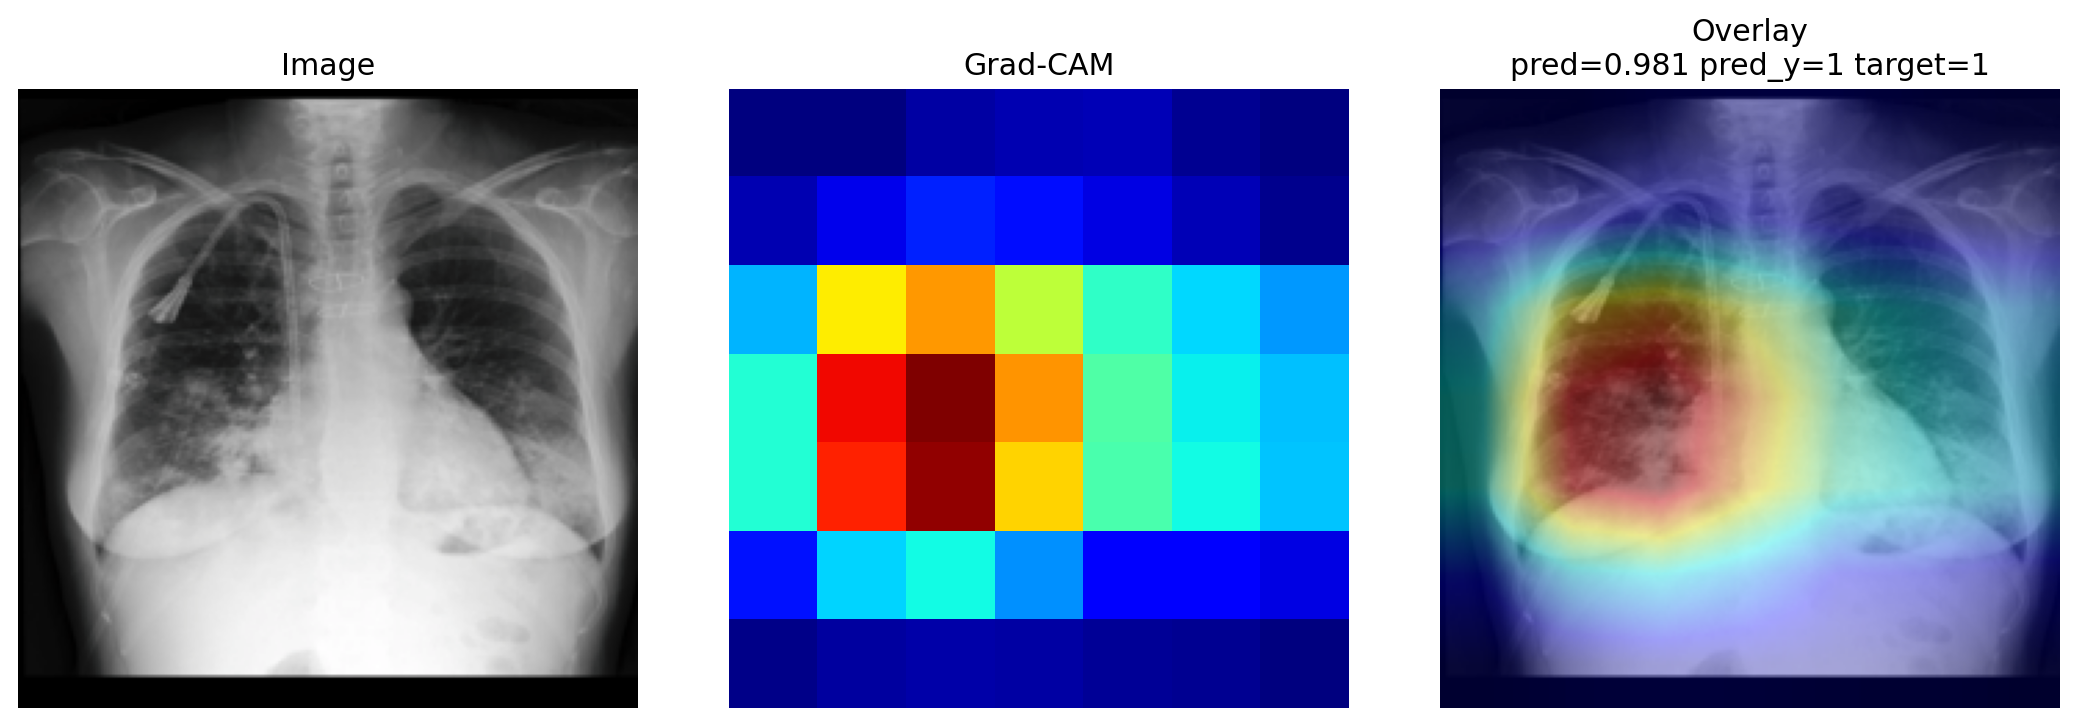
\includegraphics[width=\textwidth]{images/gradcam_tp2.png}
        \vspace{2pt}
        \small (b) True positive. Diffuse activation aligns with radiographic abnormalities.
    \end{minipage}

    \vspace{6pt}

    \begin{minipage}{0.48\textwidth}
        \centering
        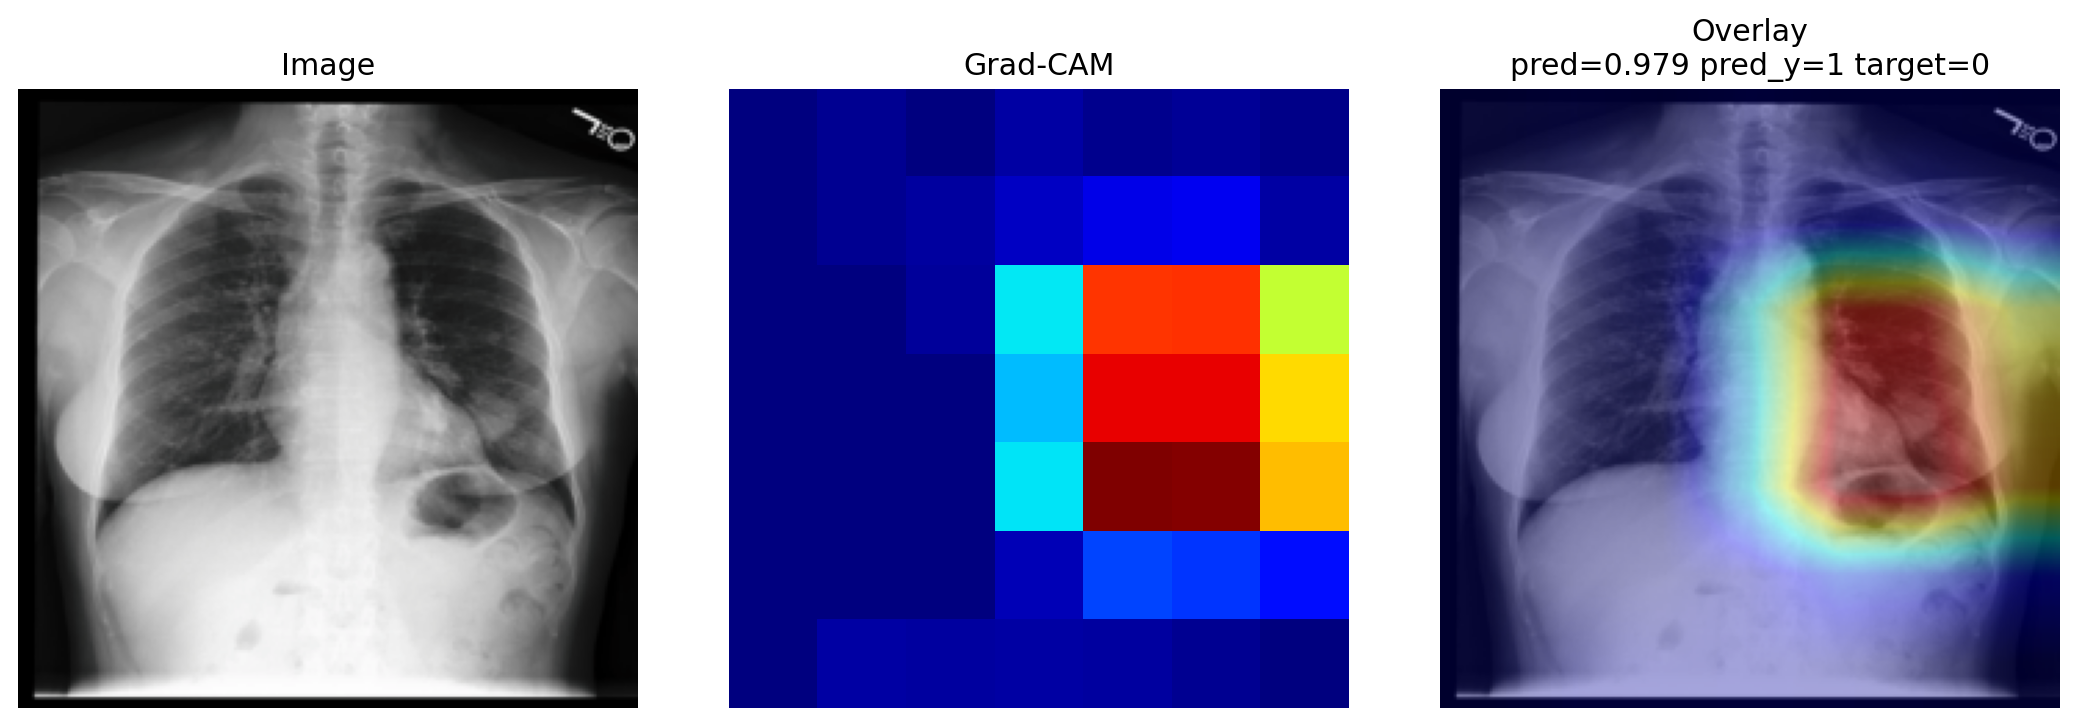
\includegraphics[width=\textwidth]{images/gradcam_fp.png}
        \vspace{2pt}
        \small (c) False positive. Attention is placed on non-pathological or non-specific abnormal structures.
    \end{minipage}
    \hfill
    \begin{minipage}{0.48\textwidth}
        \centering
        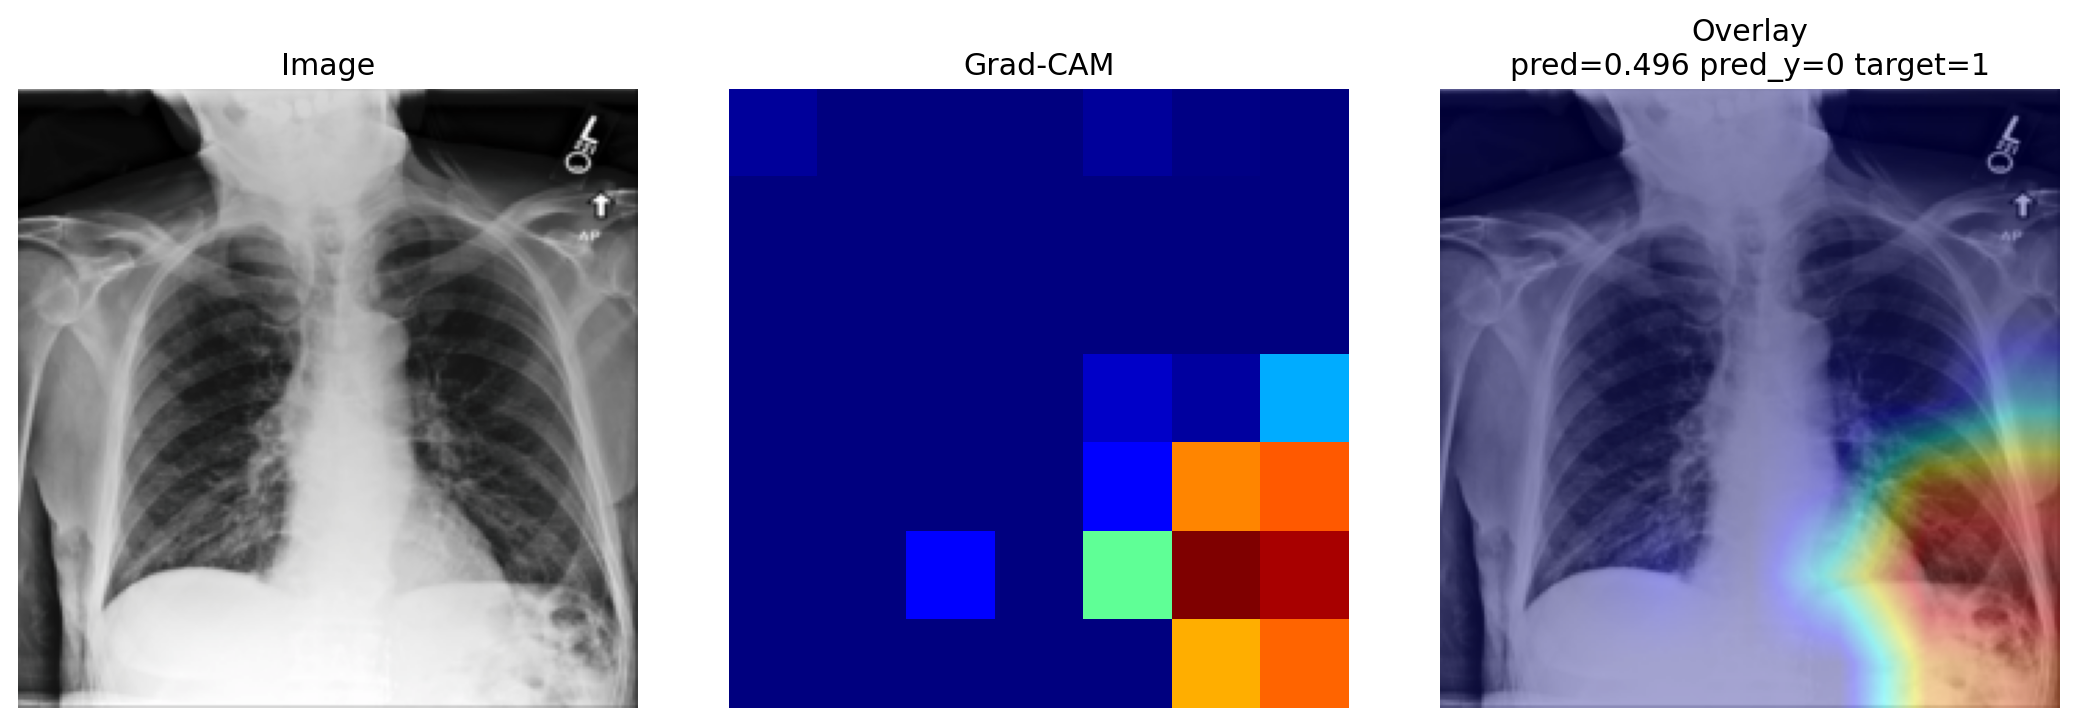
\includegraphics[width=\textwidth]{images/gradcam_fn.png}
        \vspace{2pt}
        \small (d) False negative. Weak activation over subtle or diffuse pathological regions.
    \end{minipage}

    \caption{Grad-CAM visualizations for representative cases from the image model. Heatmaps indicate regions contributing most strongly to predictions. Correct predictions align with plausible lung regions, while errors highlight sensitivity to confounders and missed subtle findings.}
    \label{fig:gradcam_cases}
\end{figure}

In correctly classified cases, the model attends to lung fields and regions consistent with pneumonia. False positives suggest sensitivity to confounding or non-specific visual patterns, while false negatives indicate difficulty in detecting subtle or diffuse abnormalities.

These qualitative examples do not serve as proof of general behavior by themselves, but they provide useful explanatory context for the quantitative results. In particular, the Grad-CAM cases suggest that correct predictions tend to arise when radiographic abnormalities are sufficiently localized or visually salient, whereas errors occur in settings where the visual evidence is weak, distributed, or confounded by other thoracic structures. This interpretation is consistent with the idea that the image model is strong when pneumonia presents with relatively clear radiographic correlates, but less reliable in ambiguous cases.

\section{Hard-Negative Analysis}

A stratified analysis based on CheXpert abnormality labels yielded 686 studies after restricting evaluation to rows with available abnormality-label information. This subset contained 392 pneumonia-positive studies, 132 normal negatives, and 162 abnormal negatives without pneumonia. For pneumonia versus normal negatives, AUROC was 0.769 for the image model and 0.755 for the multimodal model, with AUPRC values of 0.914 and 0.906, respectively. For pneumonia versus abnormal negatives, AUROC decreased to 0.632 for the image model and 0.599 for the multimodal model, with AUPRC values of 0.810 and 0.792. The corresponding AUROC differences between abnormal-negative and normal-negative subsets were approximately $-0.137$ for the image model and $-0.156$ for the multimodal model, with similar reductions observed for AUPRC.

This analysis is one of the most informative secondary results in the thesis. It shows that the apparent difficulty of the task depends strongly on how the negative class is defined. When negative cases are relatively normal, both image-based models separate them from pneumonia more effectively. When the negative class is restricted to other abnormal studies, discrimination falls substantially. This suggests that the true challenge is not simply to distinguish pneumonia from normal radiographs, but to distinguish pneumonia from other radiographic abnormalities with partially overlapping visual patterns.

The hard-negative analysis also provides a useful interpretation for both the Grad-CAM failure cases and the limited multimodal gain. If the dominant difficulty lies in differentiating among multiple abnormal thoracic presentations, then triage variables alone may not be sufficiently specific to resolve that ambiguity. In this setting, it is plausible that the image representation remains the dominant source of useful information, while the structured clinical features add limited incremental signal. Notably, the drop in AUROC between normal-negative and abnormal-negative subsets is somewhat larger for the multimodal model than for the image-only model, suggesting that fusion does not resolve this ambiguity in the present formulation.